\documentclass[11 pt]{scrartcl}
\usepackage[header, margin, koma, stylish]{tyler}
\usepackage{csquotes}

\pagestyle{fancy}
\fancyhf{}
\fancyhead[l]{EECS 127 Notes}
\fancyhead[r]{Tyler Zhu}
\cfoot{\thepage}

\begin{document} 
\title{\Large EECS 127: Optimization Models in Engineering}
\author{\large Tyler Zhu}
\date{\large\today}

\maketitle 

\begin{center}
\begin{displayquote}
    \emph{"A good stock of examples, as large as possible, is indispensable for a thorough understanding of any concept, and when I want to learn something new, I make it my first job to build one."} \\ \begin{flushright} \emph{– Paul Halmos}.  \end{flushright}
\end{displayquote}
\end{center}


These are course notes for the Spring 2021 rendition of EECS 127, Optimization Models in Engineering, taught by Professor Laurent El Ghaoui.

\tableofcontents 

\newpage

\section{Tuesday, January 19th}
\subsection{Introduction}
In this course, we'll be talking primarily about \emph{optimization}. 
A standard form of optimization is the following: 
\[ p^* = \min_\vx f_0(\vx)\quad \text{subject to: } f_i(\vx) \leq 0,\; i=1,\dots, m,\] 
where 
\itemnum
    \ii vector $\vx\in \RR^n$ is the \emph{decision variable}; 
    \ii $f_0: \RR^n \to \RR$ is the \emph{objective} function, or \emph{cost}; 
    \ii $f_i: \RR^n\to \RR$, $i=1,\dots, m$, represent the \emph{constraints}; 
    \ii $p^*$ is the \emph{optimal value}. 
\itemend

Realistically, $\vx = [x_1\; \dots\; x_n]$ represents different decisions, i.e. $x_2$ would be our decision at time $t=2$. 
Also note that we can easily solve instead to maximize some $r(x)$ by setting $f_0(x) = -r(x)$. 
This above setup is known as the \emph{standard form}. 

Oftentimes we will have multiple optimal solutions to the constraint, in which case any $x^* \in \arg\min f_0(x)$ for which $f_i(x^*) \leq 0, i=1, \dots, m$ is satisfied acts as an optimizer.

In this class, we're not as concerned with algorithms for optimization, but more so translating problems from the real world into this language. 

\begin{example}[Least-squares regression]
A classic example in machine learning is when we have a given vector $y$ and we're trying to express it as a linear function of an input vector $z$, i.e. data points. 
The goal is the solve the objective 
\[ \min_x \sum_{i=1}^m (y_i - x^\T z^{(i)})^2\] 
where 
\itemnum
    \ii $z^{(i)}\in \RR^n$, $i=1, \dots, n$ are data points; 
    \ii $y\in \RR^m$ is a ``response'' vector; 
    \ii $x^\T z$ is the scalar product $z_1x_1+\dots + z_nx_n$ b/w the two vectors $x,z \in \RR^n$. 
\itemend

One example of constraints we could be working with are $x\geq 0$ and $x^\T \one = 1$, which corresponds to modeling a discrete distribution.

\end{example}

\begin{example}[Support Vector Machines (SVMs)]
In SVMs, we instead are trying to optimize a ``hinge'' loss, i.e. 
\[ \min_{x,b} \sum_{i=1}^m \max(0, 1-y_i(x^\T z^{(i)} + b))\] 
where 
\itemnum
    \ii $z^{(i)}\in \RR^n$, $i=1, \dots, n$ are data points; 
    \ii $y\in \{-1, 1\}^m$ is a \emph{binary} response vector; 
    \ii $x^\T z + b = 0$ defines a ``separating hyperplane'' in data space. 
\itemend

We could imagine that our points are colored green and red.
Then at a conceptual level, we're trying to create a hyperplane that separates our data points into two different classes as clearly as possible. 
Once we find the best $x,b$, we can predict the binary output $\hat{y}$ corresponding to a new point's predicted class.
\end{example}

While we just gave a few machine learning examples which were problems without constraints, we can often use optimization to act on certain situations. 
One example is energy production. 
There's a \textbf{lot} of other ones. 


\subsection{Optimization Problems}
There is more nomenclature we need to know: 
\itemnum
    \ii \emph{Feasible set}, i.e. the set of possible values satisfying the constraints. 
    \ii \emph{Unconstrained minimizer}:$x_0$, i.e. minimizing the cost function without constraints. 
    \ii \emph{Optimal Point}: $x^*$. 
    \ii \emph{Level sets} of objective functions, i.e. sets $\{x | R(x) = c\}$ for some $c$. 
    \ii \emph{Sub-level sets}, i.e. sets $\{ x | R(x) \leq c\}$ for some $c$. 
\itemend
Usually our optimal points will be some intersection with the smallest level sets and the feasible set. 

Similar to neural networks, we can have an issue in optimization of local vs. global optimal points. 
A point $z$ is \emph{locally optimal} if there exists a value $R>0$ such that $z$ is optimal for problem 
\[ \min_x\; f_0(x) \text{ s.t. } f_i(x) \leq 0,\;  i=1, \dots, m \text{ and } |x_i - z_i| \leq R,\; i=1, \dots, n.\] 

A local minimizer $x$ minimizes $f_0$, but only compared to nearby points on the feasible set. 
The value of the objective function at that point is \emph{not} necessarily the (global) optimal value of the problem. 
Locally optimal points might be of no practical interest to the user. 
Visually, you could imagine that we could find ourselves in certain pits that locally seem like optima but globally are far from it. 

Due to these problems (and others), often times even coming up with any minimizer can be difficult. 
However, there's a special class of problems called \emph{convex problems} which have the nice property that \emph{all} local optimums are also global optimums.
Usually your objective function when plotted looks something like a bowl, i.e. there's a single point at the bottom which is the previously mentioned global optimum.

\begin{figure}[!htb]
    \centering
    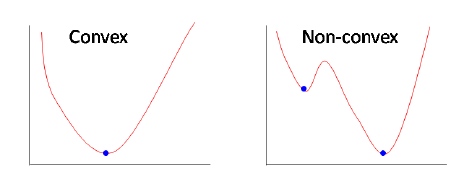
\includegraphics[scale=0.6]{convexnonconvex.png}
    \caption{Convex and Non-convex functions}
\end{figure}

Funny enough, even though most problems are non-convex, we could find a convex function that lower bounds our objective function and hope its global optimum is a decent solution to our original objective. 
Pushing this further, if we could find the tightest convex function which is a lower bound (think convex hulls), then its optimal point \emph{is} the same as our original's! 
It looks like we just turned a hard problem into a much easier one, but we unfortunately have no idea how to find this convex-hull. 
Back to square one. 

\subsection{Course Outline}

In this course, we shall deal specifically with convex optimization problems with special structure, such as: 
\itemnum
    \ii Least-Squares (LS)
    \ii Linear Programs (LP)
    \ii Convex Quadratic Program (QP)
    \ii Second-order cone programs (SOCP)
\itemend

For such specific models, very efficient solution algorithms exist with high quality implementations/software (CVX, for example). 
Most of the problems we come across can be categorized into one of the above structures, as we'll come to see. 

A large part of our time will be spent talking about affine subspaces, and normal vectors to hyperplanes to geometrically construct feasible sets. 

We'll also discuss a few non-convex problems that come up often in the real world: 
\itemnum
    \ii \emph{Boolean/integer optimization}: $x_i\in \{0,1\}^n$; some variables are constrained to be Boolean or integers. Convex optimization can be used for getting (sometimes) good approximations. 
    \ii \emph{Cardinality-constrained problems}: we seek to bound the number of non-zero elements in a vector variable. Convex optimization can be used for getting good approximations. 
    \ii \emph{Non-linear programming}: usually non-convex problems with differentiable objective and functions. Algorithms provide only local minima. 
\itemend

It goes without saying that most (but not all) non-convex problems are \emph{hard}!

For example, let's look at boolean optimization. We would like to solve $\min_{\vx} c^\T \vx$ subject to $A\vx \leq b$ and $\vx\in \{0,1\}^n$. 
One way of relaxing this into a problem that's easier to solve is to consider instead $\vx \in [0,1]^n$, i.e. going from discrete to continuous feasible set.
This is an important question because this allows us to do sparsity and feature-selection. 

What this course is for: 
\itemnum
    \ii Learning to model and efficiently solve problems arising in Engineering, Management, Control, Finance, ML, etc. 
    \ii Learning to prototype small- to medium- sized problems on numerical computing platforms. 
    \ii Learning basics of applied linear algebra, convex optimization.
\itemend

What this course is NOT: 
\itemnum
    \ii A course on mathematical convex analysis.
    \ii A course on details of optimization algorithms. 
\itemend

Here's a high level overview of what we're talking about: 
\itemnum
    \ii Linear algebra models 
    \itemnum
        \ii Vectors, projection theorem, matrices, symmetric matrices.
        \ii Linear equation, least-squares and minimum-norm problems.
        \ii Singular value decomposition (SVD), PCA, and related optimization problems. 
    \itemend
    \ii Convex optimization models 
    \itemnum
        \ii Convex sets, convex functions, convex problems. 
        \ii Optimality conditions, duality. 
        \ii Special convex models: LP, QP, SOCP.
    \itemend
    \ii Applications 
    \itemnum
        \ii Machine Learning.
        \ii Control.
        \ii Finance.
        \ii Engineering desisgn.
    \itemend
\itemend

There will only be six homeworks in this course.

\newpage
\section{Thursday, January 21st}
Today's lecture went pretty fast and sped through sections, so likewise these notes are pretty rough. 
Also I don't have time to add pictures (unless I rip them off from somewhere), so I hope you have Beth Harmon level visualization powers. 

\subsection{Introduction}
We usually write vectors in column format, i.e. 
\[ x = \colvec{4}{x_1}{x_2}{\vdots}{x_n}.\] 
Element $x_i$ is the $i$th component, and the number $n$ of components is the \emph{dimension} of $x$. 
Importantly, in math, we always 1-index, not 0-index. 

We can use vectors for example in bag of words frequency matching.

\begin{example}[Time series]
    We can model a time series, i.e. the evolution of a physical or economical quantity. 
    We can represent it like $x = [x(1)\; x(2)\; \dots\; x(T)]^\T\in\RR^T$ where each $x(k)$ is the value of the quantity at time $k$.

    One example of a model for time series is an ``auto-regressive'' model, where we assume that the output depends linearly on certain previous terms and some stochasticity (i.e. error). 
    For example, if we think it only depends on the previous two days, we could write that 
    \[ x_t \approx \alpha_1 x_{t-1} + \alpha_2 x_{t-2} + \text{error}.\]
\end{example}

Vectors have a few special properties, in that the operations of sum, difference, and scalar multiplication all hold and are closed, i.e. that they return other vectors. 
These properties define a \emph{vector space}. 
The simplest example is $\Xcal = \RR^n$. 

From a vector space $\Xcal$, a nonempty subset $\mathcal{V}$ of $\Xcal$ is a \emph{subspace} if, for any scalars $\alpha, \beta$, 
\[ x,y \in \mathcal{V} \implies \alpha x + \beta y \in \mathcal{V}.\] 
For example, the set of all possible linear combinations of vectors in $S = \{x^{(1)}, \dots, x^{(m)}\}$ forms a subspace called the \emph{span} of $S$, denoted as $\spn(S)$. 

Finally, given two subspaces $\Xcal, \Ycal$ in $\RR^n$, the \emph{direct sum} of $\Xcal, \Ycal$, denoted by $\Xcal\oplus \Ycal$, is the set of vectors of the form $x+y$ with $x\in \Xcal, y\in \Ycal$. 
One can easily check that $\Xcal\oplus\Ycal$ is a subspace. 

We also have the familiar concepts of linear independence and hence the \emph{basis} for a subspace $\Scal$, the smallest set of vectors which spans $\Scal$, whose cardinality defines the dimension of the subspace.

\begin{definition}[Affine sets]
    An affine set is a set of the form 
    \[ \Acal = \{x\in \Xcal\; | x = v+x^{(0)}, v\in \Vcal\},\] 
    where $x^{(0)}$ is a given point and $\Vcal$ is a given subspace of $\Xcal$. 
    Subspaces are affine spaces containing the origin (i.e. $x^{(0)}$ is the origin). 
\end{definition}

Naturally, a \emph{line} is a one-dimensional affine set. 
We start with some point $x_0$ which hinges the line, and then some vector $v$ which determines the direction (i.e. including all multiples of it). 

Quick quiz: how many values do we need to uniquely determine lines in 2D? 
You might think it's 2, but we need to identify the vertical line as well, so it's 3. 
Think of $ax+by+c=0$. 

One question we might have is how do we measure the \emph{size} of a vector; norms are the answer to this question. 
In short, a \emph{norm} simply assigns real numbers to vectors in a consistent manner, i.e. it satisfies the following properties: 
\begin{definition}[Norm]
    A function $\|\cdot\|$ from $\Xcal$ to $\RR$ is a \emph{norm} if 
    \begin{enumerate}
        \ii $\|x\| \geq$ for all $x\in \Xcal$, and $\|x\| = 0$ iff $x = 0$; 
        \ii $\|x+y\| \leq \|x\| + \|y\|$, for any $x,y\in \Xcal$ (triangle inequality); 
        \ii $\|\alpha x\| = \alpha \|x\|$, for any scalar $\alpha$ and any $x\in \Xcal$.
    \end{enumerate}
\end{definition}

A classic example of a norm which we'll use often are the $\ell_p$ norms, defined by 
\[ \|x\|_p := \left(\sum_{k=1}^n |x_k|^p \right)^{1/p}, \quad 1\leq p < \infty.\] 

We will primarily use three norms: 
\itemnum
    \ii For $p=2$, we obtain the standard Euclidean length 
    \[ \|x\|_2 = \sqrt{\sum_{k=1}^n x_k^2},\] 
    \ii or $p=1$ which gives the sum-of-absolute-values length (or Manhattan distance) 
    \[ \|x\|_1 = \sum_{k=1}^n |x_k|.\] 
    \ii When $p=\infty$, it defines the $\ell_\infty$ norm (max absolute value norm) 
    \[ \|x\|_{\infty} = \max_{k=1,\dots, n} |x_k|.\] 
    \ii The cardinality of a vector $x$ is often called the $\ell_0$ (pseudo-) norm, which
\itemend

\subsection{Inner product}
Inner products are interesting since we can think of vectors now as functions acting on other vectors, i.e. like $\cyc{x, \cdot}$. 
\begin{definition}[Inner product]
    An \emph{inner product} on a (real) vector space $\Xcal$ is a real-valued function which maps pairs $x,y\in \Xcal$ into a scalar denoted by $\cyc{x,y}$. 
    The inner product satisfies the following axioms (for $x,y,z\in \Xcal$ and scalar $\alpha$):
    \begin{align*}
        \cyc{x,x} &\geq 0;  \\
        \cyc{x,x} &= 0 \text{ iff } x = 0;  \\
        \cyc{x+y,x} &= \cyc{x,z} + \cyc{y,z};  \\
        \cyc{\alpha x,y} &= \alpha \cyc{x,y};  \\
        \cyc{x,y} &= \cyc{y,x}.
    \end{align*}
\end{definition}

A vector space with an inner product is called an \emph{inner product space}, and the standard inner product in $\RR^n$ is the row-column product of two vectors, 
\[ \cyc{x,y} = x^\T y = \sum_{k=1}^n x_ky_k.\] 
The inner product induces a norm given by $\|x\| = \sqrt{\cyc{x,x}}$ (which you may notice is identical to the $\ell_2$-norm in $\RR^n$). 

With inner products, we can define the angle $\theta$ between two vectors $x,y$ by 
\[ \cos \theta = \dfrac{x^\T y}{\|x\|_2\|y\|_2},\]
which results from doing some easy geometry. 
This lets us characterize when $x,y$ are \emph{orthogonal} (i.e. $\theta = \pm 90^\circ$), and when $x,y$ are \emph{parallel} (i.e. $\theta = 0^\circ, \pm 180^\circ$). 

Since $|\cos\theta| \leq 1$, we easily get the following inequality. 
\begin{theorem}[Cauchy-Schwarz Inequality]
    For vectors $x,y\in \RR^n$, 
    \[ |x^\T y| \leq \|x\|_2 \|y\|_2\] 
    where equality holds when $x = \alpha y$ for scalar $\alpha$ (i.e. when $|\cos\theta| = 1$). 
\end{theorem}

We also have the following generalization with $\ell_p$ norms. 
\begin{theorem}[Holder's Inequality]
    For any vectors $x,y\in \RR^n$ and for any $p,q \geq 1$ such that $1/p + 1/q = 1$, it holds that 
    \[ |x^\T y| \leq \sum_{k=1}^n|x_ky_k| \leq \|x\|_p \|y\|_q.\] 
\end{theorem}

\subsection{Maximization of inner product over norm balls}
Let's solve our first optimization problem and discuss maximizing the inner product over norm balls. 
We're trying to solve the optimization problem 
\[ \max_{\|x\|_p\leq 1} x^\T y.\] 

For $p=2$, we can use the Cauchy-Schwarz inequality to get $|x^\T y\| \leq \|x\|_2 \|y\|_2$, where equality holds when $x = \alpha y$. 
Since $\|x\|_2 \leq 1$ and we want the largest positive value, we should take 
\[ x_2^* = \frac{y}{\|y\|_2},\]
so $\max_{\|x\|_2\leq 1} x^\T y = \|y\|_2$. 

For $p=\infty$, each entry of $x$ should be $\pm 1$ to satisfy the norm condition, which then maximizes the inner product by making everything positive, so 
\[ x_\infty^* = \sgn(y).\] 
So $\max_{\|x\|_\infty \leq 1} x^\T y = \|y\|_1$. 

For $p=1$, we simply set 
\[ [x_1^*] = \begin{cases} \sgn(y_i)\quad &\text{ if }i = m \\ 0 \quad &\text{ o/w } \end{cases},\quad i= 1,\dots, n,\] 
where $m$ is the index of an entry in $y$ which has maximum absolute value. 
Then $\max_{\| x\|_1 \leq 1} x^\T y = \|y\|_\infty$. 

Notice that all of these results are in line with what we'd expect by applying Holder's inequality to each case.


\subsection{Orthogonalization and Projections} 
In our favorite vector space $\RR^2$, two vectors are perpendicular when they have a dot product 0.
For generic inner product spaces, we say that two vectors $x,y$ in an inner product space $\Xcal$ are \emph{orthogonal} if $\cyc{x,y} = 0$, which we denote by $x\perp y$. 
Nonzero vectors are \emph{mutually orthogonal} if they are pairwise orthogonal.
It is a simple exercise to show that mutually orthogonal vectors are linearly independent.

Given a subset $\Scal$ of an inner product space $\Xcal$, a vector $x\in \Xcal$ is orthogonal to $\Scal$ if $x\perp s$ for all $s\in \Scal$. 
The set of vectors orthogonal to $\Scal$ is called the \emph{orthogonal complement} of $\Scal$, and is denoted by $\Scal^\perp$. 

\begin{theorem}[Orthogonal Decomposition]
    If $\Scal$ is a subspace of an inner-product space $\Xcal$, then any vector $x\in \Xcal$ can be uniquely written as the sum of an element in $S$ and an element in $S^\perp$, i.e. 
    \[ \Xcal = \Scal \oplus \Scal^\perp \quad \text{ for any subspace } \Scal\subseteq \Xcal.\]
\end{theorem}

Now we will talk about projections. 
The idea of projection is central in optimization, which is finding a point on a given set that is closest (in norm) to a given point. 


We have an important theorem concerning projections.
\begin{theorem}[Projection Theorem]
    Let $\Xcal$ be an inner product space, $x$ be a given element in $\Xcal$, and $\Scal$ a subspace of $\Xcal$. 
    Then, there exists a unique vector $x^*\in \Scal$ which is the solution to the problem 
    \[ \min_{y\in\Scal} \|y-x\|.\] 
    Moreover, a necessary and sufficient condition for $x^*$ being the optimal solution for this problem is that $x^*\in \Scal,\; (x-x^*)\perp \Scal$. 
\end{theorem}

Let $p\in \RR^n$ be a given point. 
We want to compute the Euclidean projection $p^*$ of $p$ onto a line $L = \{x_0 + \spn(u)\}$, $\|u\|_2 = 1$. 
%For example, we can write this simply as 

Now say we want to solve the harder problem of projecting onto a span of vectors, say $\Scal = \spn(x^{(1)}, \dots, x^{(d)})\subseteq \Xcal$. 
By the projection theorem, we can convert this into a system of equations and solve. 


\subsection{Functions and maps}
In this class, we usually reserve the term \emph{function} to denote $f: \RR^n\to \RR$, and use the term \emph{map} when $f: \RR^n \to \RR^m$ and $m > 1$.

A \emph{linear} function is simply a function that perserves scaling and additivity, i.e. that 
\begin{align*}
    f(\alpha x) &= \alpha f(x) \quad\forall x\in \RR^n, \alpha\in\RR \\ 
    f(x + y) &= f(x) + f(y) \quad\forall x,y\in \RR^n.
\end{align*}

The gradient of a function can be intepreted in the context of level sets. 
Geometrically, the gradient of $f$ at a point $x_0$ is a vector $\nabla f(x_0)$ perpendicular to the contour line of $f$ at level $\alpha = f(x_0)$, pointing from $x_0$ outwards the $\alpha$-sublevel set (i.e. points towards higher values of the function). 

\newpage
\section{Tuesday, January 26th: Matrices and Linear Maps}

\subsection{Matrix Basics}
In this class, we will use the convention that if $A$ is a data matrix, then every column of $A$ is a single data point. 
Also, note that $x^\T Ay = y^\T A^\T x$, since the inner product is symmetric and the result is a scalar. 
This will be useful later on when we discuss duality. 

There's many ways we can think of a matrix-vector product. 
Let $A\in \RR^{m,n}$ with columns $a_1, \dots, a_n\in \RR^m$, and $b\in \RR^n$ a vector. 
Then we can define the product by 
\[ Ab = \sum_{k=1}^n a_k b_k,\] 
which is essentially just a weighted sum of the columns of $A$ with the elements of $b$ as coefficients. 

We can do the same definition for multiplication on the right by $A$. 
Let $\alpha_1, \dots, \alpha_m$ be the rows of $A$. 
If instead we had some $c\in \RR^m$, we can multiply on the left by it's transpose to get 
\[ c^\T A = \sum_{k=1}^m c_k\alpha_k^\T,\]
which says that this is a weighted sum of the rows $\alpha_k$ of $A$ using the elements of $c$ as coefficients. 


From matrix-vector products, we can then define matrix products.
We can view a matrix $A\in \RR^{m,n}$ in two different ways; either as a collection of columns or rows.
\[ A = \rowvec{4}{a_1}{a_2}{\dots}{a_n}, \text{   or   } A = \colvec{4}{\alpha_1^\T}{\alpha_2^\T}{\vdots}{\alpha_m^\T},\] 
where $a_1, \dots, a_n\in \RR^m$ denote the columns of $A$ and $\alpha_1^\T, \dots, \alpha_m^\T\in \RR^n$ denote the rows of $A$. 

We have three main interpretations of matrix-matrix products. 
One is obtained by letting $A$ act as a linear map on the columns of $B$, where $B = \RR^{n,p}$ and $B = [b_1\;\dots\;b_p]$. 
This gives 
\[ AB = A\rowvec{3}{b_1}{\dots}{b_p} = \rowvec{3}{Ab_1}{\dots}{Ab_p}.\] 

Similarly, we can also view the product as the linear map $B$ operating on the rows of $A$, which gives 
    \[ AB = \colvec{3}{\alpha_1^\T}{\vdots}{\alpha_m^\T} B = \colvec{3}{\alpha_1^\T B}{\vdots}{\alpha_m^\T B}.\] 

Finally, we can also write $AB$ as a sum of \emph{dyadic} matrices (i.e. rank one matrices of the form $uv^\T$).
Letting $\beta_i^\T$ denote the rows of $B$, we can write 
\[ AB = \sum_{i=1}^n a_i \beta_i^\T.\] 

\subsection{Matrices as linear maps}
Assume that $A$ is an $m\times n$ matrix unless stated otherwise. 
Recall that we can interpret matrices as \emph{linear maps}, i.e. maps where $f(ax+by) = af(x) + bf(y)$ for scalars $a,b$. 
Affine maps are simply linear functions plus a constant, i.e. $f(x) = Ax+b$. 

Also recall that we have the familiar concepts of range, rank, and nullspace. 
Specifically, the set of linear combinations of the columns $a_i$'s of a matrix $A$ are of the form $Ax$, for $x\in \RR^n$. 
We call this the \emph{range} of $A$, and denote it as 
\[ \Rcal(A) = \{Ax | x\in \RR^n\}.\] 
The dimension of $\Rcal(A)$ (i.e. cardinality of a basis for $A$ or the number of lin. ind. rows of $A$) is called the \emph{rank} of $A$.
We also have that $\rank(A) = \rank(A^\T)$. 

On the other hand, the null space of $A$ gives the vectors which are mapped to zero by $A$ (i.e. the \emph{kernel}) and is denoted by 
\[ \Ncal(A) = \{x \in \RR^n | Ax = 0\}.\] 

The null space of a matrix gives you the ``ambiguity'' of the solutions to $Ax = 0$. 
For any two solutions $Ax = 0$ and $Ay=0$, $A(x+y) = A(x-y) = 0$, so $x+y, x-y \in \Ncal(A)$ for example.

Importantly, $\Rcal(A^\T)$ and $\Ncal(A)$ are mutually orthogonal subspaces, i.e. $\Ncal(A)\perp \Rcal(A^\T)$, meaning that every vector in one space is orthogonal to every vector in the other.
This leads us to the following fundamental theorem. 

\begin{theorem}[Fundamental Theorem of Linear Algebra]
    For any given matrix $A \in \RR^{m,n}$, it holds that $\Ncal(A) \perp \Rcal(A^\T)$ and $\Rcal(A) \perp\Ncal(A^\T)$, hence 
    \begin{align*}
        \Ncal(A) \oplus \Rcal(A^\T) &= \RR^n \\ 
        \Rcal(A) \oplus \Ncal(A^\T) &= \RR^m.
    \end{align*}
    Consequently, we can decompose any vector $x\in \RR^n$ into a vector in the range of $A^\T$ and another in the nullspace of $A$: 
    \[ x = A^\T\xi + z, \quad z\in \Ncal(A).\] 
    Similarly, we can decompose any vector $w\in \RR^m$ into a vector in the range of $A$ and another in the nullspace of $A^\T$:
    \[ w = A\varphi + \zeta, \quad \zeta \in \Ncal(A^\T).\] 
\end{theorem}

This theorem makes much more sense geometrically. 
We did a derivation of least squares using the fundamental theorem which is cool, and I might put in when I find time. 

\subsection{Matrix Concepts}
Things we didn't cover in lecture that I need to review and note on (for my own sake): determinants, inverses, similar matrices, eigenvalues and diagonalizability, ... 

Some matrices with special structure: 
\itemnum
    \ii Square, diagonal, triangular (upper or lower). 
    \ii Symmetric: a square matrix $A$ such that $A = A^\T$. 
    \ii Orthogonal: a square matrix $A$ such that $AA^\T = A^\T A = I$. 
    These are interesting since this implies $A^{-1} = A^\T$. 
    So for any vector $x$, $\|Ax\|_2^2 = x^\T A^\T Ax = x^\T x = \|x\|_2^2$, so orthogonal matrices don't change the norm of $x$. 
    Hence, they actually represent rotations. 
    \ii Dyads (i.e. ``outer products''): matrices of the form $uv^\T$. 
    Let $A = uv^\T$. Then the $(i,j)$-th entry of $A$ is 
    \[ A_{ij} = e_i^\T(uv^\T) e_j = (e_i^\T u)(v_j^\T e_j) = u_iy_j,\] 
    (where $e_i, e_j$ are the elementary vectors) which is reminiscent of the inner product. 
\itemend

Outer products are quite useful in practice, for multiple reasons. 
If you have a data matrix like a time series, and observe that it is close to an outer product, then you can tell that you have factors which are scaled versions of each other. 

We can also find what the rank of an outer product is. 
If $A = xy^\T$, then an element of its range looks like $Az = (xy^\T)z = x(y^\T z)$. 
This last term is a scalar (as it's an inner product), so all outputs are scaled versions of $x$, and thus $A$ is rank one. 
In fact, all dyads are rank one. 

\newpage
\section{Thursday, January 28th}

\subsection{Orthogonalization: Gram-Schmidt}
Recall that a basis $(u_i)_{i=1}^n$ is said to be \emph{orthogonal} if $u_i^\T u_j = 0$ for $i\not= j$. 
If $\|u_i\|_2 = 1$, the basis is said to be \emph{orthonormal}.


Orthogonalization is the process where we find an orthonormal basis of the span of given vectors (which could be linearly dependent!). 
Specifically, given vectors $a_1, \dots, a_k\in \RR^n$, an orthogonalization procedures computes vectors $q_1, \dots, q_n\in \RR^n$ such that 
\[ S:= \spn \{a_1, \dots, a_k\} = \spn\{q_1,\dots,q_r\},\] 
where $r = \dim S$ and $(q_1, \dots, q_r)$ is an orthonormal basis for $S$. 

One useful concept for this process is that of a projection onto a line. 
We have a point $a\in \RR^n$ which we want to project onto a line $L(q) := \{tq : t\in \RR\}$, where $q$ is a unit vector in $\RR^n$. 
This amounts to solving the optimization problem 
\[ \min_{t\in \RR} \|a-tq\|_2\] 
for the closest point on $L(q)$ to $a$. 
The resulting vector $a_{\proj} := t^* q$ ($t^*$ being the optimal value) is this projection onto the line $L(q)$. 
This optimization problem has a simple solution (by geometry):
\[ a_{\proj} = (q^\T a) q.\] 

A simple interpretation of this is that we are \emph{removing the component} of $a$ along $q$, since $a-a_\proj$ and $a_\proj$ are orthogonal. 
Gram-Schmidt uses this idea to then create a set of vectors which are orthogonal to each other. 
The big idea is to first orthogonalize each vector w.r.t. the previous ones then normalize it to have norm one. 

\begin{theorem}[Gram-Schmidt Procedure]
    Let $a_1, \dots, a_n$ be linearly independent. 
    The Gram-Schmidt procedure below will output an orthonormal basis for $\spn\{a_1, \dots, a_n\}$. 
    \itemnum
        \ii Set $\tilde{q}_1 = a_1$. 
        \ii Normalize: set $q_1 = \tilde{q}_1/\|\tilde{q}_1\|_2.$
        \ii Remove component of $q_1$ in $a_2$:: set $\tilde{q}_2 = a_2 - (a_2^\T q_1) q_1$. 
        \ii Normalize: set $q_2 = \tilde{q}_2/\|\tilde{q}_2\|_2$. 
        \ii Remove component of $q_1, q_2$ in $a_3$: set $\tilde{q}_3 = a_3 - (a_3^\T q_1)q_1 - (a_3^\T q_2)q_2$. 
        \ii Normalize: set $q_3 = \tilde{q}_3/\|\tilde{q}_3\|_2$. 
        \ii etc.
    \itemend
\end{theorem}

We start by projecting each $a_i$ onto the previous normalized basis vectors, which makes it orthogonal to them. 
Then we normalize so that our basis becomes orthonormal.

This is well-defined, since if $\tilde{q}_i$ is ever 0, this means that the vectors are linearly dependent, which we assumed against. 
This means we can easily modify the above to produce a basis in the linearly dependent case; simply skip $a_i$ if the result $\tilde{q}_i$ turns out to be 0. 

\subsection{QR Decomposition}
The basic goal of QR decomposition is to factor a matrix as a product of two matrices which hopefully have simple structure to exploit. 
This will make it easier to solve equations $Ax = y$, since we can instead analyze $Cx = z$ and then $Bz = y$ as  
\[ Ax = B(Cx) = Bz = y.\] 
For example, if we could factor $A = BC$ where $B$ is some rotation, then we could easily solve this by taking its inverse rotation. 

The QR decomposition is just the Gram-Schmidt procedure applied to the columns of the matrix, with the result applied in matrix form. 

Consider an $m\times n$ matrix $A = (a_1, \dots, a_n)$ with columns $a_i$, and assume the columns are linearly independent. 
Then $A$ is full column-rank, so each step of G-S can be written as 
\[ a_i = (a_i^\T q_1) q_1 + \dots + (a_i^\T q_{i-1})q_{i-1} + \|\tilde{q}_i\|_2 q_i, \quad i=1,\dots, n\] 
where recall that $\tilde{q}_i = a_i - (a_i^\T q_1)q_1 - \dots - (a_i^\T q_{i-1})q_{i-1}$ (the remaining components of $a_i$, per se). 
We write this as 
\[ a_1 = r_{i1}q_1 + \dots + r_{i, i-1} q_{i-1} + r_{ii} q_i, \quad i = 1,\dots, n,\] 

where $r_{ij} = (a_i^\T q_j)$ for $1\leq j \leq i-1$ and $r_{ii} = \| \tilde{q}_i \|_2$. 

Since we got this output from G-S, we know the $q_i$'s form an orthonormal basis, so the matrix $Q = (q_1, \dots, q_n)$ satisfies $Q^\T Q = \II_n$ (i.e. is an \emph{orthonormal} matrix). 
The QR decomposition thus allows us to write the matrix in a \emph{factored} form 
\[ 
    A = QR,\quad Q = \rowvec{3}{q_1}{\dots}{q_n}, \quad R = 
    \bpm r_{11} & r_{12} & \dots & r_{1n} \\ 
         0      & r_{22} &       & r_{2n} \\ 
         \vdots &        & \ddots& \vdots \\ 
         0      &        &  0    & r_{nn} 
   \epm 
\]
where $Q$ is an $m\times n$ matrix with $Q^\T Q = \II_n$ and $R$ is $n\times n$ upper-triangular. 

With this decomposition, this makes it very efficient to solve linear equations, since any equation of the form $Ax = y$ can be written as $QRx = y$. 
We can then multiply by $Q^\T$ to get $Rx = Q^\T y$, and $R$ is upper-triangular, so we can efficiently solve this using back-substitution.


When the columns of $A$ are not independent, G-S simply skips over any zero vectors $\tilde{q}_j$ that we encounter. 
In matrix form, this means we obtain a factorization $A = QR$, with $Q \in \RR^{m\times r}$, $r = \rank(A)$, and $R$ having an upper staircase form like 
\[ R = 
    \bpm 
        * & * & * & * & * & * \\
        0 & 0 & * & * & * & * \\
        0 & 0 & 0 & 0 & 0 & * 
    \epm
\]

This is just as simple for us to solve with back-substitution, but we can also permute the columns of $R$ so that we bring all the pivot entries to thhe front. 

\subsection{Kernels in Machine Learning}
Recall that in least-squares, our training problem is solving the optimization problem 
\[ \min_{w, b} \Lcal(X^\T w + b\cdot 1, y),\] 
where the pairs of poinits $(X_i, y_i)$ with $X_i\in\RR^n, y_i\in \RR$ form our training set.

Our predictions are then given by $\hat{y}(x) = w^\T x +  b$ once we find these optimal $w,b$.
This means we can compute an error between the \emph{actual} measured output $y_i$ with our predictions $\hat{y}_i$, which forms our loss function that we try to optimize:

\[ \min_{w,b} \sum_{i=1}^n (y_i - (w^\T x_i + b))^2.\] 

The shape of our data is $X = \rowvec{3}{x_1}{\dots}{x_m}$, i.e. an $n\times m$ matrix, so 
\[ X^\T w + b\cdot 1 = \colvec{3}{x_1^\T \cdot w + b}{\vdots}{x_m^\T \cdot w+b} .\] 
Analyzing the term $X^\T w$ is the key to understanding the impact of kernels.

Suppose we simplify our problem to 
\[ \min_w \Lcal (X^\T w) + \la \| w\|_2^2\] 
where $\la > 0$ is a penalty/regularization term on our weights trying to force our training process to find a more ``robust example for weights $w$.'' 
It helps account for noise in your dataset, so that small changes in the $x_i$ won't result in large changes in our loss. 

Let's analyze the simple case $m = 2$ (\# of data points) and $n = 3$ (dimension of data points). 
Invoking the fundamental theorem of linear algebra, we can write our weight vector in terms of a vector in the span of our $x_1, x_2$, i.e. $w = Xv + r$ where $v\in \spn\{x_1, \dots, x_m\}$ and $r\in \Ncal(X^\T)$, so $X^\T r = 0$. 
So $X^\T w = X^\T X v+ X^\T r = X^\T X v$, which let's us rewrite the optimization problem as 
\[ 
    \min_{w,v} \Lcal[X^\T X v, y] + \la v^\T X^\T X v.  
\]
In other words, we've converted the optimization in terms of $X$ instead into an optimization in terms of the matrix $X^\T X$. 
We refer to this matrix as the \emph{kernel} matrix $K = X^\T X$, or the Gram matrix of our data. 
Note that 
\[ K_{ij} = e_i^\T K e_j = e_i^\T X^\T X e_j = x_i^\T x_j = \cyc{x_i, x_j}.\]
This inspires us to think of other inner products that aren't just the usual scalar product $\cyc{x_i, x_j} = x_i^\T x_j$. 
We could use nonlinear products instead which let use use richer models on transformed data instead. 


\newpage
\section{Tuesday, February 2nd}

Today is about symmetric matrices. 
\subsection{Symmetric Matrices} 
Recall that a square $n\times n$ matrix $A$ is \emph{symmetric} if $A = A^\T$. 
The set of symmetric $n\times n$ matrices is a subspace of $R^{n,n}$, and is denoted by $\SS^n$. 

\begin{example}[Sample covariance Matrix]
    \label{ex:cov}
    For one dimensional data $z_1, \dots, z_m\in \RR$, we can define the mean and variance of the data as 
    \[ \hat{z} = \frac{1}{m} \sum_{i=1}^m z_i \] 
    \[ \si^2 = \frac{1}{m} \sum_{i=1}^m (z_i-\hat{z})^2.\] 
    
    We can extend this notion to multi-dimensional points, which results in an important symmetric matrix we will see many times: the covariance matrix. 
    
    The covariance matrix is a way for us to understand the variance along any direction $u$ ($\|u\|_2=1$). 
    Let $x_1, \dots, x_m \in \RR^n$, which has sample mean $\hat{x} = \frac 1m \sum_{i=1}^m x_i$. 
    If we project our points $x$ onto this line by using $x' = (x^\T u)u$, we reduce this to the previous one dimensional case and analyze the mean and variance again.
    This creates ``scores'' of our points along the line $u$ defined by $z_i = (x_i-\hat{x})^\T u$. 
    Then following the same procedure from before, we can compute variance as 
    \begin{align*}
        \si^2(u) &= \frac{1}{m}\sum_{i=1}^m (z_i - \hat{z})^\T (z_i-\hat{z}) \\ 
                 &= \frac{1}{m}\sum_{i=1}^m u^\T (x_i-\hat{x}) (x_i-\hat{x})^\T u  \\ 
                 &= u^\T C u
    \end{align*}
    where $C= \frac{1}{m}\sum_{i=1}^m (x_i-\hat{x}) (x_i-\hat{x})^\T$ is the covariance matrix.
    From this, one can see that we can use it to compute arbitrary sample variances.
\end{example}

\begin{example}[Hessian matrix]
    The Hessian of a twice differentiable function $f: \RR^n \to \RR$ at a point $x$ is the matrix containing the second derivates of the function at that point. 
    It is given by 
    \[ H_{ij} = \dfrac{\pd^2 f(x)}{\pd x_i \pd x_j}, \; 1\leq i,j\leq n.\] 
    We usually denote the Hessian by $\nabla^2 f(x)$. 
    Since the second-derivative is the same regardless of order of derivative, $H_{ij} = H_{ji}$, so it is symmetric. 
\end{example}

As a quick aside, we can talk about quadratic functions being written as matrices and vectors. 
Supposes we have a quadratic function 
\[ q(x) = x_1^2 + 2x_1x_2 + 3x_2^2 + 4x_1 + 5x_2+6,\]
which has Hessian 
\[ H = \bbm 2&2 \\ 2 & 6 \ebm.\] 

We can also write the monomials as 
\[ x_1^2 + 2x_1x_2 + 3x_2^2 = \frac 12 x^\T H x.\] 
Hence, any quadratic function can be written as the sum of a quadratic term involving the Hessian, and an affine term: 
\[ q(x) = \frac 12 x^\T H x + c^\T x + d, \quad c^\T = [4\; 5],\; d = 6.\] 


We can finally get to this most important result, which states that every symmetric matrix is orthogonally similar to a diagonal matrix. 

\begin{theorem}[Spectral Theorem]
    Let $A$ be a symmetric $n\times n$ matrix and let $\la_i\in \RR, (i=1, \dots, n)$ be its eigenvalues with multiplicty. 
    Then there exists a set of orthogonal vectors $u_i \in \RR^n$, $i=1,\dots, n$ such that $Au_i = \la_i u_i$. 
    Equivalently, there exists an orthogognal matrix $U = \rowvec{3}{u_1}{\cdots}{u_n}$ (i.e. $UU^\T = U^\T U = \II_n$) such that 
    \[ A = U\Lambda U^\T = \sum_{i=1}^n \la_i u_i u_i^\T, \quad \Lambda = \diag(\la_1, \dots, \la_n).\] 
\end{theorem}

In other words, $A$ can be written as the weighted sum of dyads which are mutually orthogonal. 

Also talked about Rayleigh quotients and matrix gain. 

\subsection{Positive-Semidefinite Matrices}
\begin{definition}[PSD]
    A symmetric matrix $A\in \SS^n$ is said to be \emph{positive semidefinite} (PSD) if the associated quadratic form is nonnegative, i.e., 
    \[ x^\T A x \geq 0, \quad \forall x \in \RR^n.\]

    If, moreover, 
    \[ x^\T A x > 0, \quad \forall x\in \RR^n\setminus\{0\},\] 
    then $A$ is said to be \emph{positive definite} (PD). 
    We denote a symmetric positive semidefinite (resp. positive definite) matrix by $A\succeq 0$ (resp. $A\succ 0$). 
\end{definition}

Some immediate properties are that a PSD matrix is actually positive definite if and only if it is invertible. 
Also, it holds that 
\[ A \succeq 0 \iff \la_i(A) \geq 0,\; i=1, \dots, n.\] 
\[ A \succ   0 \iff \la_i(A) > 0,\; i=1, \dots, n.\] 

We then talked about Matrix square-root, Cholesky decomp, and PSD's with ellipsoids. 
Schur complements are on the homework.

\subsection{Principal Component Analysis}

The motivation behind PCA is that if we have a low-dimensional data set existing in a high-dimensional space, then we should instead view it from an angle where the ``variance'' of thhe data is highest. 
In other words, we want to project our data onto a direction which maximizes the resulting variance of our points, since that lets us tell the points apart the most. 

When we do this, recall that the variance of the projections of our points onto a direction $u$ is given by the covariance matrix (Example~\ref{ex:cov})
This gives us the optimization problem 
\[ \max_u\; u^\T C u: \quad \|u\|_2 = 1\] 
where $C$ is the empirical covariance matrix and we impose the unit vector constraint so that the optimization is actually tractable. 

To solve this, we can look at the spectral decomposition of $C$ given by 
\[ C = \sum_{i=1}^p \la_i u_i u_i^\T,\] 
with $\la_1 \geq \dots \geq \la_p$ and $U = [u_1,\dots, u_p]$ is orthogonal ($U^\T U = I$). Then a solution to the quadratic form 
\[ \max_{u: \|u\|_2=1} \; u^\T C u\] 
is $u^* = u_1$ where $u_1$ is the eigenvector of $C$ that corresponds to the largest eigenvalue $\la_1$ as we discussed before. 

Later we will see how to arrive at this using SVD. 


\newpage
\section{Thursday, February 4th}
PCA and SVD. 

\begin{theorem}[SVD]
    woohoo (to be added)
    \label{thm:svd}
\end{theorem}


\newpage
\section{Tuesday, February 9th}
\subsection{Motivation for Linear Equations}
Linear equations are one of the most basic form of relationship among variables in an engineering problem. 
There's all sorts of applications of linear equations that come up in science, and they form the building block for many other optimization methods, so it's important to know how to solve them.

Here is an example of a system in 3 equations in 2 unknowns: 
\begin{align*}
    x_1 + 4.5x_2 &= 1 \\ 
    2x_1 + 1.2x_2 &= -3.2  \\
    -0.1x_1 + 8.2x_2 &= 1.5.
\end{align*}

We can write this in vector format as $Ax=y$, where 
\[ A = \bbm 1 & 4.5 \\ 2 & 1.2 \\ -0.1 & 8.2 \ebm, \quad y = \colvec{3}{1}{-3.2}{1.5}.\] 
Solutions are $x\in \RR^2$ which satisfy the equation. 
In this case, the equation has no solution, i.e. the system is \emph{infeasible}.

We then went over a lot of examples. 
I prefer theory so I did not take notes on them.

\subsection{Set of Solutions of Linear Equations}
Our general setup is that we want to solve the linear equation 
\[ Ax = y, \quad A \in \RR^{m,n}.\] 

There are many issues we concern ourselves with, such as existence and uniqueness of solutions, or the characterization of the \emph{solution set} 
\[ S = \{x\in \RR^n : Ax=y\}.\] 
Notice that $Ax$ always lies in $\Rcal(A)$, so $S\not= 0 \iff y \in \Rcal(A)$. 
Hence, there is a solution if and only if $\rank([A\; y]) = \rank(A)$. 

When existence is satisfied, the set of solutions is the affine set 
\[ S = \{\bar{x} + Nz, z\in \RR^{n-r} \},\] 
where $\bar{x}$ is any vector such that $A\bar{x} = y$, $r = \rank(A)$, and $N \in \RR^{n, n-r}$ is a matrix whose columns span the nullspace of $A$ (hence $AN = 0$). 

Geometrically, the null space represents the span of the ``free variables'' in the solutions.

Finding the solution set in the above manner can be useful in optimization. We can use this by turning our usual optimization problem into an unconstrained one, i.e. 
\[ \min_x f_0(x) :\; Ax = b \implies \min_z f_0(x_0 + Nz),\] 
using notation from above. 

\subsection{Solving Linear Systems}
We can also use SVD to easily analyze our linear equation system.
As usual, suppose we're solving $Ax = y$ where $A\in \RR^{m,n}$ and $y\in \RR^m$. 
If $A = U\tilde{\Sigma} V^\T$ is the SVD of $A$ (see Theorem~\ref{thm:svd}), then $Ax = y$ is equivalent to 

\[ U\tilde{\Sigma} V^\T x = y \implies \tilde{\Sigma} V^\T x = U^\T y \implies \tilde{\Sigma} \tilde{x} = \tilde{y},\] 
where $\tilde{x} = V^\T x, \tilde{y} = U^\T y$. 

In other words, we're using $U$ and $V$ to rotate our inputs and outputs to make the system diagonal (as per the usual SVD interpretation). 
Since $\tilde{\Sigma}$ is a diagonal matrix 
\[ \tilde{\Sigma} = \bbm \Sigma & 0_{r, n-r} \\ 0_{m-r, r} & 0_{m-r, n-r} \ebm,\quad \Sigma = \diag(\si_1, \dots, \si_r) \succ 0,\]

this makes the system very easy to solve or analyze.
Note that $\Ncal(A) = m-r$. 

Let's analyze the resulting system $\tilde{\Sigma}\tilde{x} = \tilde{y}$, which reduces to 
\begin{align*}
    \si_i \tilde{x}_i &= \tilde{y}_i \quad i = 1, \dots, r \\ 
    0 &= \tilde{y}_i \quad i = r+1, \dots, m.
\end{align*}

Clearly we need $\tilde{y}_i$ to be zero for its last $m-r$ components, which happens when $y\in \Rcal(A)$. 
Otherwise the solution set is empty. 

If $y\in \Rcal(A)$, then we can solve for $\tilde{x}$ with our first set of conditions: $\tilde{x}_i = \tilde{y}_i/\si_i$ for $i = 1, \dots, r$, with the last $n-r$ components being free (which correspond to elements in the nullspace of $A$).

When $A$ is full column rank, it has trivial nullspace and hence there is a unique solution. 

\begin{example}
    Suppose we have a system $Ax = y$ with 
    \[ A = \bbm \si_1 & 0 & 0 \\ 0 & \si_2 & 0 \\ 0&0&0 \\ 0&0&0\ebm, \quad y=\colvec{4}{y_1}{y_2}{y_3}{y_4}.\]
    This system has no solution if $(y_3, y_4) \not= 0$. If $y_3=y_4 = 0$ so that $y\in \Rcal(A)$, we then get the solution sest $S = \{x_0 + Nz : z\in \RR^2\}$ with 
    \[ x_0 = \colvec{4}{y_1/\si_1}{y_2/\si_2}{0}{0},\quad N = \bbm 0&0\\0&0\\1&0\\0&1\ebm.\] 
\end{example}

Finally, we can also use QR decomposition to analyze a linear system. 
The idea is to reduce the system to a triangular one and then solve using ``back-substitution.'' 
For example, if $A$ is square and $A = QR$ with $Q^\T Q = I_n$, then $Ax = y$ is equivalent to $Rx = \tilde{y} = Q^\T y$, which is triangular. 
Then we just have to back substitute to find a solution. 

Similarly to using SVD, we're rotating our outputs here to make the system triangular and easier to solve.

\end{document}
